% =============================================================================
% KAPITEL 4: AUSWERTUNG UND DISKUSSION
% =============================================================================

\section{Auswertung und Diskussion}
\label{chap:auswertung_diskussion}

Dieses Kapitel widmet sich der Untersuchung des Einflusses verschiedener Leitergeometrien auf die Messgenauigkeit der Stromwandler. Der Fokus liegt zunächst auf der allgemeinen Beeinflussung durch die Anordnung. Im Anschluss folgen eine detaillierte Analyse der einzelnen Außenleiter sowie eine ökonomische Bewertung der Ergebnisse.

\subsection{Einfluss der Leitergeometrie auf die Messgenauigkeit}
\label{sec:vergleich_geometrie}

Die folgenden Diagramme visualisieren die Messabweichungen der Stromwandler in Abhängigkeit vom Primärstrom sowie der Leiteranordnung. Der Vergleich erfolgt jeweils zwischen Wandlern mit identischem Nennstrom. Eine detaillierte Beschreibung der verwendeten Leiteranordnungen findet sich in Abschnitt \ref{sec:layout_geometrie}.

Zur visuellen Unterscheidung gelten in den Diagrammen folgende Konventionen
\begin{itemize}
    \item Die \textbf{Parallelanordnung} wird durch eine durchgezogene Linie in Kombination mit einem Kreissymbol dargestellt
    \item Die \textbf{Dreiecksanordnung} ist durch eine gepunktete oder gestrichelte Linie sowie ein Dreieckssymbol gekennzeichnet
    \item Die \textbf{Farbgebung} verbleibt für ein spezifisches Wandlermodell in beiden Anordnungen gleich um den direkten Vergleich zu ermöglichen
\end{itemize}
Diese Darstellungsweise erlaubt die direkte Bewertung des Geometrieeinflusses auf den jeweiligen Wandlertyp.


% --- Hier beginnt der neue Unterabschnitt für den besseren Übergang ---
\subsubsection{Analyse der Messreihe \SI{2000}{A}}

Die Untersuchung der Stromwandler bei einem Nennstrom von 2000\,A zeigt differenzierte Ergebnisse für die verschiedenen Modelle und Leiteranordnungen. Abbildung \ref{dia:2000A_zusammenfassung} stellt die Verläufe der vier Prüflinge gegenüber und verdeutlicht die Einhaltung der Genauigkeitsklasse 1 für den Großteil der Messpunkte. Der grafische Vergleich hebt hervor dass insbesondere zwei Konfigurationen deutliche Abweichungen aufweisen. Dies betrifft den Redur 13A1030.ffp in der Dreiecksanordnung sowie den Celsa ALO 10030 in der Parallelanordnung. Beide Wandler verlassen in diesen spezifischen Szenarien die vorgegebenen Toleranzbereiche.

\begin{figure}[H]
    \centering
    \includegraphics[width=1.0\textwidth]{03_Ressourcen/diagramme/dia_2000A_dreieck_parallel/dia_2000A_dreieck_parallel-Zusammenfassung_MultiCurrent.pdf}
    \caption{Zusammenfassender Vergleich der Leitergeometrien bei 2000\,A}
    \label{dia:2000A_zusammenfassung}
\end{figure}

Eine bauliche Besonderheit weist der Redur 13A1030.ffp auf. Wie in Abbildung \ref{fig:wandler_fremdfeldprotektor} zu erkennen ist befinden sich die Fremdfeldprotektoren (\gls{ffp}) an den seitlichen Flanken des Gehäuses. Diese Positionierung schirmt den Eisenkern effektiv gegen magnetische Streufelder benachbarter Leiter ab sofern diese seitlich angeordnet sind. In der parallelen Leiterführung führt dies zu normkonformen Messergebnissen da die Beeinflussung durch die Nachbarphasen minimiert wird.

\begin{figure}[H]
    \centering
    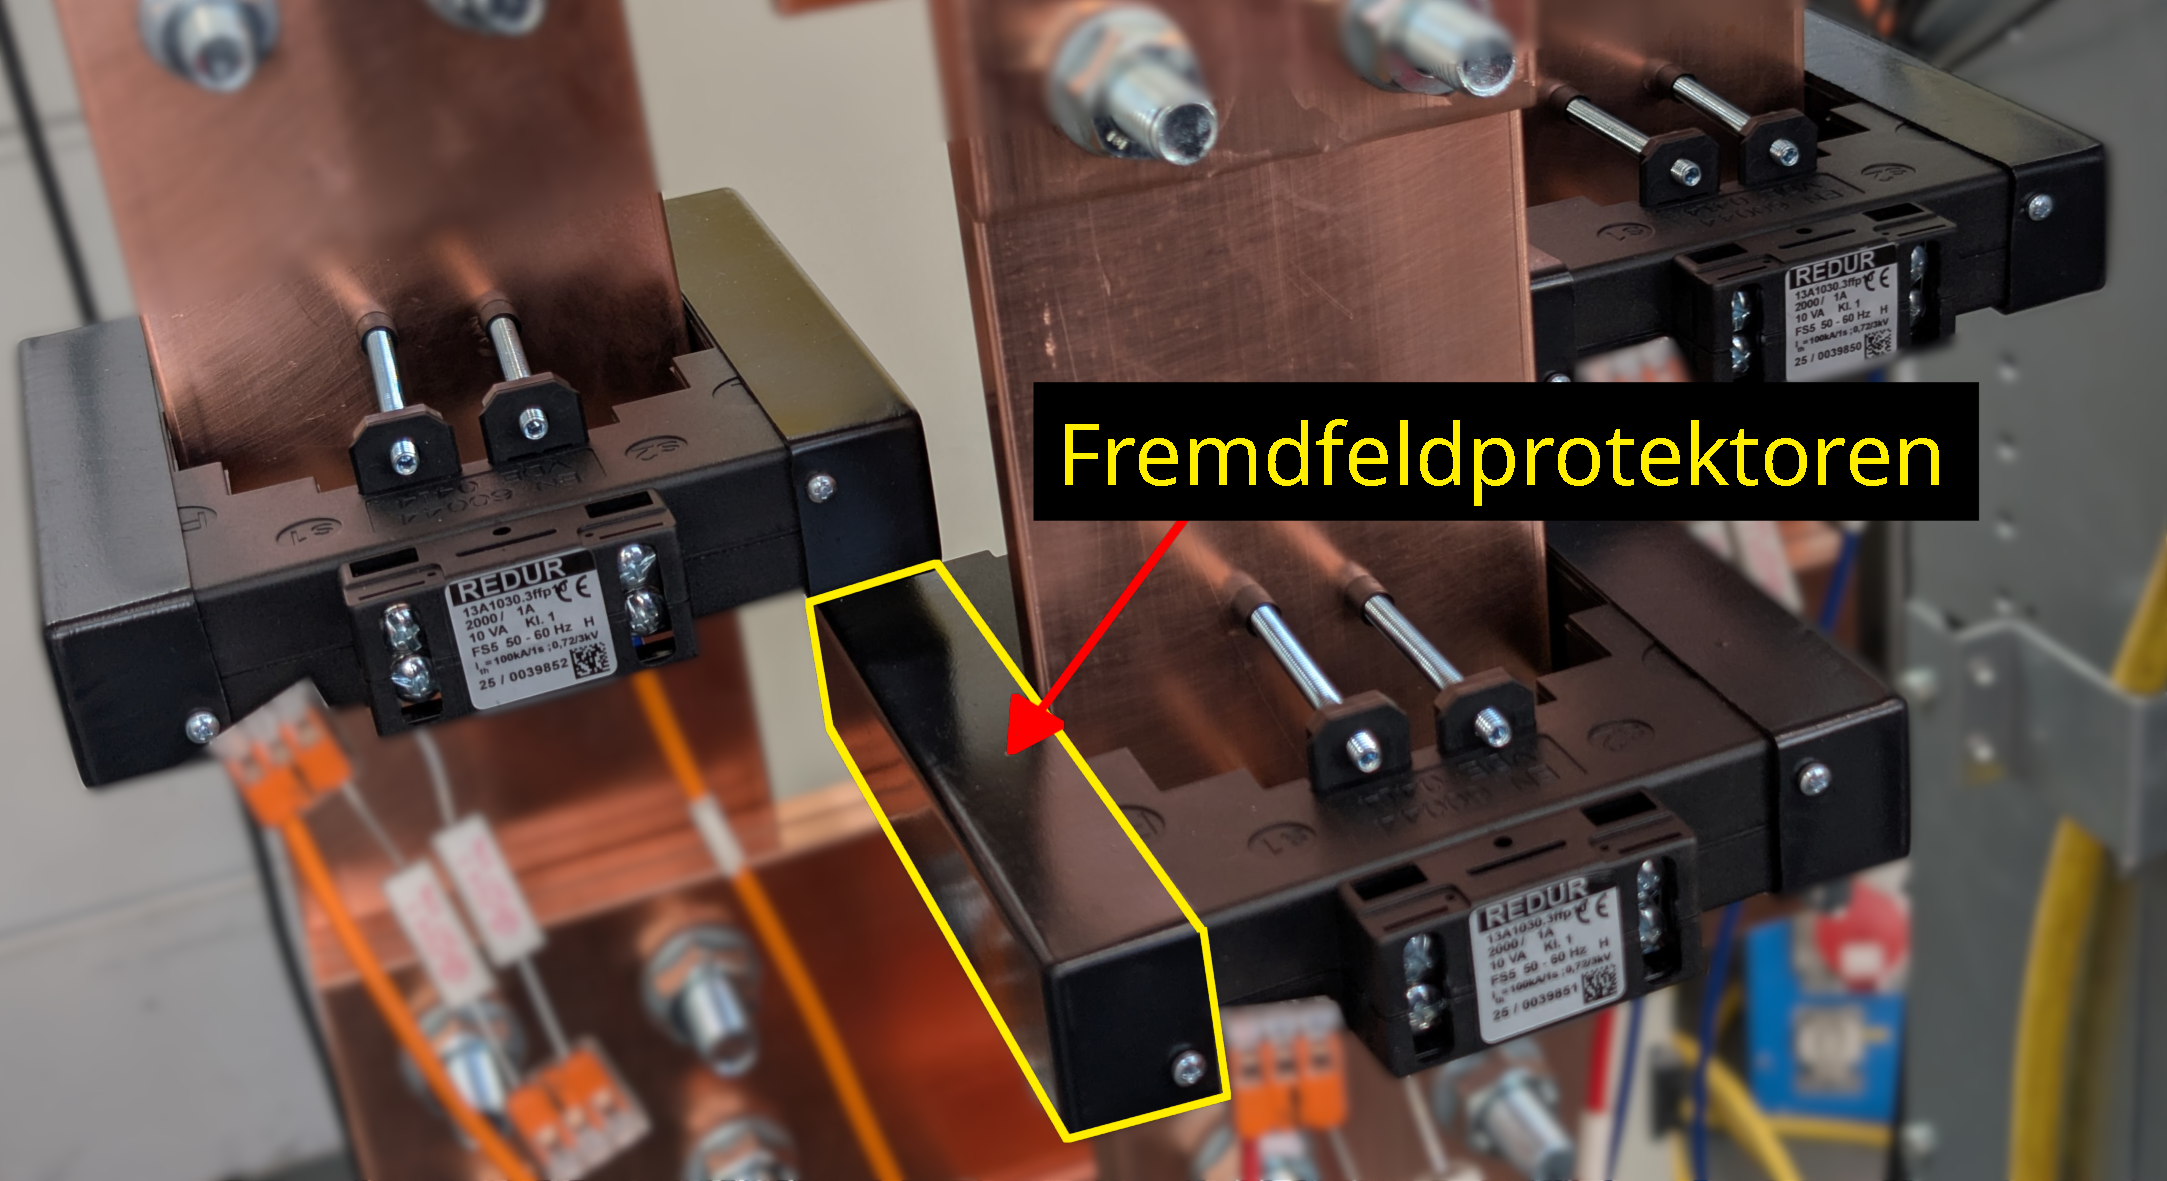
\includegraphics[width=0.8\textwidth]{03_Ressourcen/Bilder/wandler_redur_2000A_dreiecksmessung_beschriftet.pdf}
    \caption{Seitliche Fremdfeldprotektoren am Redur Wandler}
    \label{fig:wandler_fremdfeldprotektor}
\end{figure}

Die Grenzen dieser Schirmungstechnologie zeigen sich in der Dreiecksanordnung. Tabelle \ref{tab:messergebnisse_redur_2000A} listet die numerischen Ergebnisse für diesen Aufbau auf. Die Phase L2 weist bei 120\,\% des Nennstroms eine signifikante Abweichung von -1,5\,\% auf. Dieser Wert liegt außerhalb der zulässigen Toleranz der Genauigkeitsklasse 1. Ursächlich hierfür ist die fehlende magnetische Schirmung auf der Rückseite des Wandlergehäuses. In der Dreiecksgeometrie können die Magnetfelder der benachbarten Leiter an dieser ungeschützten Stelle in den Eisenkern eindringen und sättigen diesen partiell. Im Gegensatz dazu bleibt die Phase L1 mit einer Abweichung von lediglich -0,1\,\% im selben Lastpunkt weit innerhalb der Normgrenzen.

\begin{table}[H]
    \centering
    \setlength{\tabcolsep}{4pt}
    \caption{Messergebnisse: Redur 13A1030.3ffp, 2000\,A, 8,1\,$\Omega$}
    \label{tab:messergebnisse_redur_2000A}
    \small
    \begin{tabular}{
            l
            c
            S[table-format=1.3]
            S[table-format=1.2]
            S[table-format=1.3]
            S[table-format=1.2]
            S[table-format=-1.3]
            S[table-format=1.2]
            S[table-format=-1.3]
            S[table-format=2.2]
        }
        \toprule
        {}          & {}    & \multicolumn{2}{c}{5\,\% $I_n$} & \multicolumn{2}{c}{20\,\% $I_n$} & \multicolumn{2}{c}{100\,\% $I_n$} & \multicolumn{2}{c}{120\,\% $I_n$}                                   \\
        {}          & {}    & \multicolumn{2}{c}{(100\,A)}    & \multicolumn{2}{c}{(400\,A)}     & \multicolumn{2}{c}{(2000\,A)}     & \multicolumn{2}{c}{(2400\,A)}                                       \\
        \cmidrule(lr){3-4} \cmidrule(lr){5-6} \cmidrule(lr){7-8} \cmidrule(lr){9-10}
        {Geometrie} & {Ph.} & {[\%]}                          & {[A]}                            & {[\%]}                            & {[A]}                             & {[\%]} & {[A]} & {[\%]} & {[A]} \\
        \midrule
        Dreieck     & L1    & 0.473                           & 0.47                             & 0.022                             & 0.09                              & -0.120 & 2.40  & -0.121 & 2.90  \\
        Dreieck     & L2    & 0.338                           & 0.34                             & 0.088                             & 0.35                              & -0.094 & 1.88  & -1.533 & 36.79 \\
        Dreieck     & L3    & 0.471                           & 0.47                             & 0.111                             & 0.44                              & 0.126  & 2.52  & -0.070 & 1.68  \\
        \addlinespace
        Parallel    & L1    & 0.376                           & 0.38                             & 0.058                             & 0.23                              & -0.081 & 1.62  & -0.103 & 2.47  \\
        Parallel    & L2    & 0.445                           & 0.45                             & 0.111                             & 0.44                              & -0.029 & 0.58  & -0.509 & 12.22 \\
        Parallel    & L3    & 0.405                           & 0.41                             & 0.146                             & 0.58                              & 0.017  & 0.34  & -0.007 & 0.17  \\
        \bottomrule
    \end{tabular}
\end{table}

Ein gegenteiliges Verhalten zeigt sich beim Modell Celsa ALO 10030. Tabelle \ref{tab:messergebnisse_celsa_2000A} dokumentiert die Messergebnisse für diesen Wandler und belegt massive Einbrüche der Genauigkeit in der parallelen Leiteranordnung. Bereits bei Nennstrom verletzt die Phase L2 mit -2,0\,\% den zulässigen Grenzwert. Bei einer Überlast von 120\,\% steigt die Abweichung weiter auf -4,2\,\% an. Auch die Außenleiter L1 und L3 zeigen in der Parallelanordnung bei 120\,\% Last mit Werten von -2,7\,\% beziehungsweise -3,1\,\% deutliche Fehler. Die Änderung der Geometrie hin zur Dreiecksanordnung bewirkt bei diesem Modell eine substanzielle Verbesserung. Der Fehler der Phase L2 reduziert sich hierbei bei 120\,\% Last auf einen unkritischen Wert von -0,2\,\%.

\begin{table}[H]
    \centering
    \setlength{\tabcolsep}{4pt}
    \caption{Messergebnisse: Celsa ALO 10030, 2000\,A, 1,35\,$\Omega$}
    \label{tab:messergebnisse_celsa_2000A}
    \small
    \begin{tabular}{
            l
            c
            S[table-format=1.3]
            S[table-format=1.2]
            S[table-format=-1.3]
            S[table-format=1.2]
            S[table-format=-1.3]
            S[table-format=2.2]
            S[table-format=-1.3]
            S[table-format=3.2]
        }
        \toprule
        {}          & {}    & \multicolumn{2}{c}{5\,\% $I_n$} & \multicolumn{2}{c}{20\,\% $I_n$} & \multicolumn{2}{c}{100\,\% $I_n$} & \multicolumn{2}{c}{120\,\% $I_n$}                                    \\
        {}          & {}    & \multicolumn{2}{c}{(100\,A)}    & \multicolumn{2}{c}{(400\,A)}     & \multicolumn{2}{c}{(2000\,A)}     & \multicolumn{2}{c}{(2400\,A)}                                        \\
        \cmidrule(lr){3-4} \cmidrule(lr){5-6} \cmidrule(lr){7-8} \cmidrule(lr){9-10}
        {Geometrie} & {Ph.} & {[\%]}                          & {[A]}                            & {[\%]}                            & {[A]}                             & {[\%]} & {[A]} & {[\%]} & {[A]}  \\
        \midrule
        Dreieck     & L1    & 0.183                           & 0.18                             & -0.103                            & 0.41                              & -0.273 & 5.46  & -0.317 & 7.61   \\
        Dreieck     & L2    & 0.530                           & 0.53                             & -0.026                            & 0.10                              & -0.211 & 4.22  & -0.230 & 5.52   \\
        Dreieck     & L3    & 0.480                           & 0.48                             & 0.072                             & 0.29                              & -0.153 & 3.06  & -0.758 & 18.19  \\
        \addlinespace
        Parallel    & L1    & 0.196                           & 0.20                             & -0.068                            & 0.27                              & -0.477 & 9.54  & -2.671 & 64.10  \\
        Parallel    & L2    & 0.201                           & 0.20                             & -0.014                            & 0.06                              & -1.971 & 39.42 & -4.240 & 101.76 \\
        Parallel    & L3    & 0.401                           & 0.40                             & 0.083                             & 0.33                              & -0.427 & 8.54  & -3.071 & 73.70  \\
        \bottomrule
    \end{tabular}
\end{table}

Diese Abhängigkeit des Fehlers vom Primärstrom wird in Abbildung \ref{dia:2000A_celsa_zusammenfassung} grafisch aufbereitet. Das Diagramm veranschaulicht den steilen Abfall der Messkurven für die Parallelanordnung ab etwa 20\,\% des Nennstroms. Im Vergleich dazu verlaufen die Kurven der Dreiecksanordnung weitestgehend linear und verbleiben im Toleranzbereich.

\begin{figure}[H]
    \centering
    \includegraphics[width=1.0\textwidth]{03_Ressourcen/diagramme/dia_2000A_celsa_10030/dia_2000A_celsa_10030-Zusammenfassung_MultiCurrent.pdf}
    \caption{Messfehlerverlauf des Celsa ALO 10030 in Abhängigkeit vom Primärstrom}
    \label{dia:2000A_celsa_zusammenfassung}
\end{figure}

Im Gegensatz zu den Abweichungen der vorangegangenen Modelle zeigen der Celsa ALO 8030 K und der MBS ASK101.4 eine hohe Stabilität gegenüber externen Feldern. Diese Unempfindlichkeit lässt sich beim Celsa ALO 8030 K auf die Bauweise als kompensierter Wandler zurückführen wie in Abschnitt \ref{sec:kompensationswicklungen} erläutert wird. Tabelle \ref{tab:messergebnisse_celsa8030_2000A} fasst die Ergebnisse für dieses Modell zusammen. Selbst unter Volllast und Überstrom bleiben alle Phasen in beiden geometrischen Anordnungen sicher innerhalb der Klasse 1. Die maximale Abweichung tritt in der Parallelanordnung bei Phase L1 mit einem Wert von -0,4\,\% auf.

\begin{table}[H]
    \centering
    \setlength{\tabcolsep}{4pt}
    \caption{Messergebnisse: Celsa ALO 8030 K, 2000\,A, 8,1\,$\Omega$}
    \label{tab:messergebnisse_celsa8030_2000A}
    \small
    \begin{tabular}{
            l
            c
            S[table-format=1.3]
            S[table-format=1.2]
            S[table-format=-1.3]
            S[table-format=1.2]
            S[table-format=-1.3]
            S[table-format=1.2]
            S[table-format=-1.3]
            S[table-format=2.2]
        }
        \toprule
        {}          & {}    & \multicolumn{2}{c}{5\,\% $I_n$} & \multicolumn{2}{c}{20\,\% $I_n$} & \multicolumn{2}{c}{100\,\% $I_n$} & \multicolumn{2}{c}{120\,\% $I_n$}                                   \\
        {}          & {}    & \multicolumn{2}{c}{(100\,A)}    & \multicolumn{2}{c}{(400\,A)}     & \multicolumn{2}{c}{(2000\,A)}     & \multicolumn{2}{c}{(2400\,A)}                                       \\
        \cmidrule(lr){3-4} \cmidrule(lr){5-6} \cmidrule(lr){7-8} \cmidrule(lr){9-10}
        {Geometrie} & {Ph.} & {[\%]}                          & {[A]}                            & {[\%]}                            & {[A]}                             & {[\%]} & {[A]} & {[\%]} & {[A]} \\
        \midrule
        Dreieck     & L1    & 0.114                           & 0.11                             & -0.115                            & 0.46                              & -0.306 & 6.12  & -0.338 & 8.11  \\
        Dreieck     & L2    & 0.220                           & 0.22                             & -0.134                            & 0.54                              & -0.279 & 5.58  & -0.299 & 7.18  \\
        Dreieck     & L3    & 0.232                           & 0.23                             & -0.110                            & 0.44                              & -0.252 & 5.04  & -0.295 & 7.08  \\
        \addlinespace
        Parallel    & L1    & 0.134                           & 0.13                             & -0.222                            & 0.89                              & -0.354 & 7.08  & -0.428 & 10.27 \\
        Parallel    & L2    & 0.091                           & 0.09                             & -0.135                            & 0.54                              & -0.268 & 5.36  & -0.354 & 8.50  \\
        Parallel    & L3    & 0.211                           & 0.21                             & -0.055                            & 0.22                              & -0.200 & 4.00  & -0.217 & 5.21  \\
        \bottomrule
    \end{tabular}
\end{table}

Ein ähnlich robustes Verhalten bestätigt Tabelle \ref{tab:messergebnisse_mbs_2000A} für den MBS ASK101.4. Auch hier sind keine signifikanten Einflüsse durch die Leiteranordnung erkennbar. Die Messwerte liegen konstant auf einem Niveau vergleichbar mit dem Celsa 8030 K. In der Dreiecksanordnung erreicht die Phase L1 bei 120\,\% Last beispielsweise eine Abweichung von -0,3\,\% und demonstriert damit die Unempfindlichkeit dieses Modells gegenüber den untersuchten geometrischen Anordnungen.

\begin{table}[H]
    \centering
    \setlength{\tabcolsep}{4pt}
    \caption{Messergebnisse: MBS ASK101.4, 2000\,A, 8,1\,$\Omega$}
    \label{tab:messergebnisse_mbs_2000A}
    \small
    \begin{tabular}{
            l
            c
            S[table-format=1.3]
            S[table-format=1.2]
            S[table-format=-1.3]
            S[table-format=1.2]
            S[table-format=-1.3]
            S[table-format=1.2]
            S[table-format=-1.3]
            S[table-format=2.2]
        }
        \toprule
        {}          & {}    & \multicolumn{2}{c}{5\,\% $I_n$} & \multicolumn{2}{c}{20\,\% $I_n$} & \multicolumn{2}{c}{100\,\% $I_n$} & \multicolumn{2}{c}{120\,\% $I_n$}                                   \\
        {}          & {}    & \multicolumn{2}{c}{(100\,A)}    & \multicolumn{2}{c}{(400\,A)}     & \multicolumn{2}{c}{(2000\,A)}     & \multicolumn{2}{c}{(2400\,A)}                                       \\
        \cmidrule(lr){3-4} \cmidrule(lr){5-6} \cmidrule(lr){7-8} \cmidrule(lr){9-10}
        {Geometrie} & {Ph.} & {[\%]}                          & {[A]}                            & {[\%]}                            & {[A]}                             & {[\%]} & {[A]} & {[\%]} & {[A]} \\
        \midrule
        Dreieck     & L1    & 0.133                           & 0.13                             & -0.097                            & 0.39                              & -0.284 & 5.68  & -0.305 & 7.32  \\
        Dreieck     & L2    & -0.279                          & 0.28                             & -0.248                            & 0.99                              & -0.204 & 4.08  & -0.232 & 5.57  \\
        Dreieck     & L3    & 0.016                           & 0.02                             & -0.044                            & 0.18                              & -0.163 & 3.26  & -0.166 & 3.98  \\
        \addlinespace
        Parallel    & L1    & 0.134                           & 0.13                             & -0.222                            & 0.89                              & -0.353 & 7.06  & -0.428 & 10.27 \\
        Parallel    & L2    & 0.091                           & 0.09                             & -0.135                            & 0.54                              & -0.268 & 5.36  & -0.355 & 8.52  \\
        Parallel    & L3    & 0.211                           & 0.21                             & -0.056                            & 0.22                              & -0.200 & 4.00  & -0.217 & 5.21  \\
        \bottomrule
    \end{tabular}
\end{table}

\newpage


\subsubsection{Analyse der Messreihe \SI{2500}{A}}

Die Analyse der Messreihe bei \SI{2500}{A} verdeutlicht den signifikanten Einfluss der Leitergeometrie auf unterschiedliche Wandlertechnologien. Im Fokus steht der Vergleich zwischen dem kompensierten Wandler Celsa ALO 10050 K und dem Standardwandler Celsa ALO 10030 in Bezug auf ihre Stabilität in Parallel- und Dreiecksanordnungen.

\begin{figure}[H]
    \centering
    \includegraphics[width=1.0\textwidth]{03_Ressourcen/diagramme/dia_2500A_dreieck_parallel/dia_2500A_dreieck_parallel-Zusammenfassung_MultiCurrent.pdf}
    \caption{Zusammenfassender Vergleich der Leitergeometrien bei 2500\,A}
    \label{dia:2500A_zusammenfassung}
\end{figure}

Die Messergebnisse des kompensierten Wandlers Celsa ALO 10050 K belegen, dass dieser über den Großteil des Messbereichs eine hohe Genauigkeit aufweist (siehe Tabelle \ref{tab:messergebnisse_celsa10050_2500A_alle}). In der Parallelanordnung bewegt sich der Wandler fast durchgehend innerhalb der Normvorgaben. Eine Ausnahme bildet jedoch die Phase L2 im Überlastbereich (120\,\% $I_n$). Hier überschreitet der Wandler den Grenzwert mit einer Abweichung von -1,012\,\% knapp, was einem absoluten Fehlstrom von rund 30\,A entspricht.
In der Dreiecksanordnung reduziert sich dieser Messfehler auf -0,549\,\%, wodurch die Norm wieder eingehalten wird. Dies zeigt, dass selbst ein kompensierter Wandler nicht vollständig immun gegen starke externe Magnetfelder ist, die Auswirkungen jedoch im Vergleich zu Standardwandlern minimal bleiben.

\begin{table}[H]
    \centering
    \caption{Gesamtmessergebnisse: Celsa ALO 10050 K, 2500\,A, 2,8\,$\Omega$ (Alle Lastpunkte)}
    \label{tab:messergebnisse_celsa10050_2500A_alle}
    \setlength{\tabcolsep}{2pt}
    \scriptsize
    \resizebox{\textwidth}{!}{%
        \begin{tabular}{
                l
                c
                S[table-format=-1.3] S[table-format=1.2]
                S[table-format=-1.3] S[table-format=1.2]
                S[table-format=-1.3] S[table-format=1.2]
                S[table-format=-1.3] S[table-format=1.2]
                S[table-format=-1.3] S[table-format=1.2]
                S[table-format=-1.3] S[table-format=1.2]
                S[table-format=-1.3] S[table-format=2.2]
            }
            \toprule
            {}       & {}    & \multicolumn{2}{c}{5\,\%}    & \multicolumn{2}{c}{20\,\%}   & \multicolumn{2}{c}{50\,\%}    & \multicolumn{2}{c}{80\,\%}    & \multicolumn{2}{c}{90\,\%}    & \multicolumn{2}{c}{100\,\%}   & \multicolumn{2}{c}{120\,\%}                                                              \\
            {}       & {}    & \multicolumn{2}{c}{(125\,A)} & \multicolumn{2}{c}{(500\,A)} & \multicolumn{2}{c}{(1250\,A)} & \multicolumn{2}{c}{(2000\,A)} & \multicolumn{2}{c}{(2250\,A)} & \multicolumn{2}{c}{(2500\,A)} & \multicolumn{2}{c}{(3000\,A)}                                                            \\
            \cmidrule(lr){3-4} \cmidrule(lr){5-6} \cmidrule(lr){7-8} \cmidrule(lr){9-10} \cmidrule(lr){11-12} \cmidrule(lr){13-14} \cmidrule(lr){15-16}
            {Geom.}  & {Ph.} & {[\%]}                       & {[A]}                        & {[\%]}                        & {[A]}                         & {[\%]}                        & {[A]}                         & {[\%]}                        & {[A]} & {[\%]} & {[A]} & {[\%]} & {[A]} & {[\%]} & {[A]} \\
            \midrule
            Dreieck  & L1    & -0.029                       & 0.04                         & -0.186                        & 0.93                          & -0.229                        & 2.86                          & -0.255                        & 5.10  & -0.259 & 5.83  & -0.279 & 6.97  & -0.305 & 9.16  \\
            Dreieck  & L2    & 0.009                        & 0.01                         & -0.140                        & 0.70                          & -0.188                        & 2.35                          & -0.222                        & 4.44  & -0.242 & 5.44  & -0.275 & 6.87  & -0.549 & 16.47 \\
            Dreieck  & L3    & 0.102                        & 0.13                         & -0.077                        & 0.38                          & -0.126                        & 1.57                          & -0.171                        & 3.42  & -0.192 & 4.33  & -0.229 & 5.72  & -0.317 & 9.52  \\
            \addlinespace
            Parallel & L1    & 0.081                        & 0.10                         & -0.164                        & 0.82                          & -0.232                        & 2.90                          & -0.273                        & 5.45  & -0.306 & 6.89  & -0.291 & 7.28  & -0.326 & 9.77  \\
            Parallel & L2    & 0.247                        & 0.31                         & -0.104                        & 0.52                          & -0.192                        & 2.40                          & -0.238                        & 4.76  & -0.301 & 6.78  & -0.372 & 9.31  & -1.012 & 30.35 \\
            Parallel & L3    & 0.234                        & 0.29                         & -0.053                        & 0.27                          & -0.135                        & 1.68                          & -0.173                        & 3.45  & -0.199 & 4.49  & -0.197 & 4.93  & -0.264 & 7.92  \\
            \bottomrule
        \end{tabular}
    }
\end{table}

Im Gegensatz dazu zeigt der nicht kompensierte Standardwandler Celsa ALO 10030 in beiden Anordnungen massive Abweichungen, die auf eine magnetische Sättigung hindeuten (siehe Tabelle \ref{tab:messergebnisse_celsa10030_2500A_alle}). In der Parallelanordnung beginnt der Fehler bereits ab 50\,\% Nennstrom signifikant anzusteigen. Bei 100\,\% Last liegen die Abweichungen bereits zwischen -10\,\% und -16\,\%. Im Überlastbereich bei 120\,\% bricht die Genauigkeit vollständig ein: Phase L2 erreicht eine negative Abweichung von -20,565\,\%, was einem absoluten Fehlstrom von über 600\,A entspricht. Auch die Phasen L1 und L3 liegen mit -16,2\,\% bzw. -13,9\,\% weit außerhalb jeglicher Toleranzgrenzen.

Die Dreiecksanordnung zeigt hingegen... [Hier bitte deinen Text einfügen]

\begin{table}[H]
    \centering
    \caption{Gesamtmessergebnisse: Celsa ALO 10030, 2500\,A, 1,35\,$\Omega$ (Alle Lastpunkte)}
    \label{tab:messergebnisse_celsa10030_2500A_alle}
    \setlength{\tabcolsep}{2pt} % Sehr kleiner Spaltenabstand
    \scriptsize % Sehr kleine Schrift
    \resizebox{\textwidth}{!}{% Skaliert die Tabelle auf Textbreite
        \begin{tabular}{
                l
                c
                S[table-format=1.3] S[table-format=1.2]
                S[table-format=-1.3] S[table-format=1.2]
                S[table-format=-1.3] S[table-format=2.2]
                S[table-format=-2.3] S[table-format=3.2]
                S[table-format=-2.3] S[table-format=3.2]
                S[table-format=-2.3] S[table-format=3.2]
                S[table-format=-2.3] S[table-format=3.2]
            }
            \toprule
            {}       & {}    & \multicolumn{2}{c}{5\,\%}    & \multicolumn{2}{c}{20\,\%}   & \multicolumn{2}{c}{50\,\%}    & \multicolumn{2}{c}{80\,\%}    & \multicolumn{2}{c}{90\,\%}    & \multicolumn{2}{c}{100\,\%}   & \multicolumn{2}{c}{120\,\%}                                                                     \\
            {}       & {}    & \multicolumn{2}{c}{(125\,A)} & \multicolumn{2}{c}{(500\,A)} & \multicolumn{2}{c}{(1250\,A)} & \multicolumn{2}{c}{(2000\,A)} & \multicolumn{2}{c}{(2250\,A)} & \multicolumn{2}{c}{(2500\,A)} & \multicolumn{2}{c}{(3000\,A)}                                                                   \\
            \cmidrule(lr){3-4} \cmidrule(lr){5-6} \cmidrule(lr){7-8} \cmidrule(lr){9-10} \cmidrule(lr){11-12} \cmidrule(lr){13-14} \cmidrule(lr){15-16}
            {Geom.}  & {Ph.} & {[\%]}                       & {[A]}                        & {[\%]}                        & {[A]}                         & {[\%]}                        & {[A]}                         & {[\%]}                        & {[A]}  & {[\%]}  & {[A]}  & {[\%]}  & {[A]}  & {[\%]}  & {[A]}  \\
            \midrule
            Dreieck  & L1    & 0.159                        & 0.20                         & -0.107                        & 0.53                          & -0.247                        & 3.09                          & -1.678                        & 33.56  & -3.337  & 75.08  & -5.066  & 126.65 & -8.278  & 248.33 \\
            Dreieck  & L2    & 0.073                        & 0.09                         & -0.204                        & 1.02                          & -0.316                        & 3.95                          & -1.568                        & 31.35  & -1.763  & 39.67  & -1.834  & 45.85  & -1.950  & 58.49  \\
            Dreieck  & L3    & 0.182                        & 0.23                         & -0.139                        & 0.69                          & -0.256                        & 3.20                          & -1.126                        & 22.53  & -2.232  & 50.22  & -3.452  & 86.29  & -5.437  & 163.12 \\
            \addlinespace
            Parallel & L1    & -0.061                       & 0.08                         & -0.214                        & 1.07                          & -0.653                        & 8.17                          & -7.423                        & 148.46 & -10.056 & 226.26 & -12.370 & 309.25 & -16.238 & 487.15 \\
            Parallel & L2    & 0.060                        & 0.08                         & -0.117                        & 0.59                          & -2.732                        & 34.15                         & -11.571                       & 231.42 & -14.277 & 321.22 & -16.623 & 415.59 & -20.565 & 616.96 \\
            Parallel & L3    & 0.180                        & 0.23                         & 0.031                         & 0.16                          & -0.119                        & 1.48                          & -5.352                        & 107.03 & -7.856  & 176.77 & -10.099 & 252.46 & -13.862 & 415.87 \\
            \bottomrule
        \end{tabular}
    }
\end{table}


\subsubsection{Analyse der Messreihe \SI{3000}{A}}

% --- 3000 A ---
\begin{figure}[H]
    \centering
    \includegraphics[width=1.0\textwidth]{03_Ressourcen/diagramme/dia_3000A_dreieck_parallel/dia_3000A_dreieck_parallel-Zusammenfassung_MultiCurrent.pdf}
    \caption{Zusammenfassender Vergleich der Leitergeometrien bei 3000\,A}
    \label{dia:3000A_zusammenfassung}
\end{figure}


\subsubsection{Analyse der Messreihe \SI{5000}{A}}
% --- 4000 A ---
\begin{figure}[H]
    \centering
    \includegraphics[width=1.0\textwidth]{03_Ressourcen/diagramme/dia_4000A_dreieck_parallel/dia_4000A_dreieck_parallel-Zusammenfassung_MultiCurrent.pdf}
    \caption{Zusammenfassender Vergleich der Leitergeometrien bei 4000\,A}
    \label{dia:4000A_zusammenfassung}
\end{figure}


\subsubsection{Analyse der Messreihe \SI{5000}{A}}

% --- 5000 A ---
\begin{figure}[H]
    \centering
    \includegraphics[width=1.0\textwidth]{03_Ressourcen/diagramme/dia_5000A_dreieck_parallel/dia_5000A_dreieck_parallel-Zusammenfassung_MultiCurrent.pdf}
    \caption{Zusammenfassender Vergleich der Leitergeometrien bei 5000\,A}
    \label{dia:5000A_zusammenfassung}
\end{figure}






\subsection{Ökonomische Evaluation und Technologie-Ranking}
\label{sec:oekonomie_ranking}

In diesem Abschnitt werden die technischen Ergebnisse mit den Kosten der Wandler korreliert.

% === 2000 A ===
\begin{diagram}[H]
    \centering
    \includegraphics[width=0.9\textwidth]{03_Ressourcen/diagramme/dia_2000A_dreieck_parallel/dia_2000A_dreieck_parallel-Oekonomie_Ranking.pdf}
    \caption{Wirtschaftliches Ranking der Wandlertechnologien bei 2000\,A}
    \label{dia:2000A_ranking_plot}
\end{diagram}

\begin{table}[H]
    \centering
    \caption{Tabellarisches Ranking der Wandlertechnologien (2000\,A)}
    \label{tab:2000A_ranking}
    \begin{table}[H]
    \centering
    \caption{2000 A | Performance-Index | Ranking}
    \label{tab:dia_2000A_kosten_ranking}
    \begin{tabular}{p{6cm}ccccc}
        \toprule
        \textbf{Messsystem} & \textbf{\shortstack[c]{Fehler \\ Niederstrom}} & \textbf{\shortstack[c]{Fehler \\ Nennstrom}} & \textbf{\shortstack[c]{Fehler \\ Überlast}} & \textbf{\shortstack[c]{Preis \\ (€)}} & \textbf{\shortstack[c]{Fehler-Score \\ {[\%]}}} \\
        \midrule
        Celsa ALO 10030 | 2000 A \newline 1,35 $\Omega$ | Dreieck & 90,50 & 22,17 & 13,07 & 32,06 & 157,80 \\
        Celsa ALO 8030 K | 2000 A \newline 8,1 $\Omega$ | Parallel & 55,03 & 28,58 & 10,00 & 67,62 & 161,23 \\
        Celsa ALO 8030 K | 2000 A \newline 8,1 $\Omega$ | Dreieck & 59,97 & 29,13 & 9,33 & 67,62 & 166,06 \\
        Redur 13A1030.3ffp | 2000 A \newline 8,1 $\Omega$ | Parallel & 100,00 & 4,45 & 6,20 & 70,47 & 181,12 \\
        MBS ASK101.4 | 2000 A \newline 8,1 $\Omega$ | Dreieck & 52,97 & 22,61 & 7,05 & 100,00 & 182,62 \\
        MBS ASK101.4 | 2000 A \newline 8,1 $\Omega$ | Parallel & 55,06 & 28,58 & 10,02 & 100,00 & 193,65 \\
        Redur 13A1030.3ffp | 2000 A \newline 8,1 $\Omega$ | Dreieck & 97,51 & 11,81 & 17,28 & 70,47 & 197,07 \\
        Celsa ALO 10030 | 2000 A \newline 1,35 $\Omega$ | Parallel & 62,49 & 100,00 & 100,00 & 32,06 & 294,55 \\
        \bottomrule
    \end{tabular}
\end{table}
\end{table}


% Sonderfall Kosten/Volumen 2000A
\begin{diagram}[H]
    \centering
    \includegraphics[width=0.9\textwidth]{03_Ressourcen/diagramme/dia_2000A_kosten_volumen/dia_2000A_kosten_volumen-Oekonomie_Ranking.pdf}
    \caption{Wirtschaftliches Ranking unter Berücksichtigung des Volumens bei 2000\,A}
    \label{dia:2000A_ranking_volumen_plot}
\end{diagram}

\begin{table}[H]
    \centering
    \caption{Tabellarisches Ranking nach Kosten/Volumen (2000\,A)}
    \label{tab:2000A_ranking_volumen}
    \begin{table}[H]
    \centering
    \caption{2000 A | Performance-Index | Ranking}
    \label{tab:dia_2000A_kosten_volumen_ranking}
    \begin{tabular}{lcccccc}
        \toprule
        \textbf{Messsystem} & \textbf{Fehler Niederstrom [\%]} & \textbf{Fehler Nennstrom [\%]} & \textbf{Fehler Überlast [\%]} & \textbf{Preis (€) [\%]} & \textbf{Volumen (Gesamt) [\%]} & \textbf{Fehler-Score [\%]} \\
        \midrule
        Celsa ALO 10030 | 2000 A | 1,35 $\Omega$ | Dreieck & 90,50 & 22,17 & 13,07 & 32,06 & 81,45 & 239,26 \\
        Celsa ALO 8030 K | 2000 A | 8,1 $\Omega$ | Parallel & 55,03 & 28,58 & 10,00 & 67,62 & 91,20 & 252,43 \\
        Celsa ALO 8030 K | 2000 A | 8,1 $\Omega$ | Dreieck & 59,97 & 29,13 & 9,33 & 67,62 & 91,20 & 257,26 \\
        MBS ASK101.4 | 2000 A | 8,1 $\Omega$ | Dreieck & 52,97 & 22,61 & 7,05 & 100,00 & 94,15 & 276,78 \\
        Redur 13A1030.3ffp | 2000 A | 8,1 $\Omega$ | Parallel & 100,00 & 4,45 & 6,20 & 70,47 & 100,00 & 281,12 \\
        MBS ASK101.4 | PAC2 | 8,1 $\Omega$ | Parallel & 55,06 & 28,58 & 10,02 & 100,00 & 94,15 & 287,81 \\
        Redur 13A1030.3ffp | 2000 A | 8,1 $\Omega$ | Dreieck & 97,51 & 11,81 & 17,28 & 70,47 & 100,00 & 297,07 \\
        Celsa ALO 10030 | 2000 A | 1,35 $\Omega$ | Parallel & 62,49 & 100,00 & 100,00 & 32,06 & 81,45 & 376,00 \\
        \bottomrule
    \end{tabular}
\end{table}
\end{table}


% === 2500 A ===
\begin{diagram}[H]
    \centering
    \includegraphics[width=0.9\textwidth]{03_Ressourcen/diagramme/dia_2500A_dreieck_parallel/dia_2500A_dreieck_parallel-Oekonomie_Ranking.pdf}
    \caption{Wirtschaftliches Ranking der Wandlertechnologien bei 2500\,A}
    \label{dia:2500A_ranking_plot}
\end{diagram}

\begin{table}[H]
    \centering
    \caption{Tabellarisches Ranking der Wandlertechnologien (2500\,A)}
    \label{tab:2500A_ranking}
    \begin{table}[H]
    \centering
    \caption{2500 A | Performance-Index | Ranking}
    \label{tab:dia_2500A_kosten_ranking}
    \begin{tabular}{lccccc}
        \toprule
        \textbf{Messsystem} & \textbf{Fehler Nennstrom [\%]} & \textbf{Fehler Niederstrom [\%]} & \textbf{Fehler Überlast [\%]} & \textbf{Preis (€) [\%]} & \textbf{Fehler-Score [\%]} \\
        \midrule
        Celsa ALO 10050 K | 2500 A | 2,8 $\Omega$ | Dreieck & 2,22 & 26,04 & 2,31 & 100,00 & 130,57 \\
        Celsa ALO 10030 | 2500 A | 1,35 $\Omega$ | Dreieck & 23,06 & 40,36 & 30,92 & 43,67 & 138,01 \\
        Celsa ALO 10050 K | 2500 A | 2,8 $\Omega$ | Parallel  & 2,46 & 34,58 & 3,16 & 100,00 & 140,20 \\
        Celsa ALO 10030 | 2500 A | 1,35 $\Omega$ | Parallel & 100,00 & 100,00 & 100,00 & 43,67 & 343,67 \\
        \bottomrule
    \end{tabular}
\end{table}
\end{table}



% === 3000 A ===
\begin{diagram}[H]
    \centering
    \includegraphics[width=0.9\textwidth]{03_Ressourcen/diagramme/dia_3000A_dreieck_parallel/dia_3000A_dreieck_parallel-Oekonomie_Ranking.pdf}
    \caption{Wirtschaftliches Ranking der Wandlertechnologien bei 3000\,A}
    \label{dia:3000A_ranking_plot}
\end{diagram}

\begin{table}[H]
    \centering
    \caption{Tabellarisches Ranking der Wandlertechnologien (3000\,A)}
    \label{tab:3000A_ranking}
    \begin{table}[H]
    \centering
    \caption{3000 A | Performance-Index | Ranking}
    \label{tab:dia_3000A_kosten_ranking}
    \begin{tabular}{p{6cm}ccccc}
        \toprule
        \textbf{Messsystem} & \textbf{\shortstack[c]{Fehler \\ Nennstrom}} & \textbf{\shortstack[c]{Fehler \\ Überlast}} & \textbf{\shortstack[c]{Preis \\ (€)}} & \textbf{\shortstack[c]{Fehler \\ Niederstrom}} & \textbf{\shortstack[c]{Fehler-Score \\ {[\%]}}} \\
        \midrule
        Celsa ALO ALO 12070 | 3000 A \newline 1,35 $\Omega$ | Dreieck & 25,99 & 12,64 & 20,66 & 92,32 & 151,61 \\
        Celsa ALO 12070 K | 3000 A \newline 2,8 $\Omega$ | Parallel & 11,63 & 14,73 & 100,00 & 75,93 & 202,28 \\
        Celsa ALO 12070 K | 3000 A \newline 2,8 $\Omega$ | Dreieck & 13,60 & 2,98 & 100,00 & 97,23 & 213,81 \\
        Celsa ALO ALO 12070 | 3000 A \newline 1,35 $\Omega$ | Parallel & 100,00 & 100,00 & 20,66 & 100,00 & 320,66 \\
        \bottomrule
    \end{tabular}
\end{table}
\end{table}


% === 4000 A ===
\begin{diagram}[H]
    \centering
    \includegraphics[width=0.9\textwidth]{03_Ressourcen/diagramme/dia_4000A_dreieck_parallel/dia_4000A_dreieck_parallel-Oekonomie_Ranking.pdf}
    \caption{Wirtschaftliches Ranking der Wandlertechnologien bei 4000\,A}
    \label{dia:4000A_ranking_plot}
\end{diagram}

\begin{table}[H]
    \centering
    \caption{Tabellarisches Ranking der Wandlertechnologien (4000\,A)}
    \label{tab:4000A_ranking}
    \begin{table}[H]
    \centering
    \caption{4000 A | Performance-Index | Ranking}
    \label{tab:dia_4000A_kosten_ranking}
    \begin{tabular}{lccccc}
        \toprule
        \textbf{Messsystem} & \textbf{Fehler Nennstrom [\%]} & \textbf{Fehler Überlast [\%]} & \textbf{Fehler Niederstrom [\%]} & \textbf{Preis (€) [\%]} & \textbf{Fehler-Score [\%]} \\
        \midrule
        Celsa ALO ALO 12070 | 3000 A | 0,0 $\Omega$ | Dreieck & 18,43 & 27,07 & 89,60 & 17,79 & 152,89 \\
        Celsa ALO 12070 K | 3000 A | 0,0 $\Omega$ | Parallel  & 9,64 & 5,06 & 89,00 & 100,00 & 203,70 \\
        Celsa ALO 12070 K | 4000 A | 10,8 $\Omega$ | Dreieck  & 10,11 & 6,11 & 100,00 & 100,00 & 216,22 \\
        Celsa ALO ALO 12070 | 3000 A | 0,0 $\Omega$ | Parallel & 100,00 & 100,00 & 85,77 & 17,79 & 303,56 \\
        \bottomrule
    \end{tabular}
\end{table}
\end{table}


% === 5000 A ===
\begin{diagram}[H]
    \centering
    \includegraphics[width=0.9\textwidth]{03_Ressourcen/diagramme/dia_5000A_dreieck_parallel/dia_5000A_dreieck_parallel-Oekonomie_Ranking.pdf}
    \caption{Wirtschaftliches Ranking der Wandlertechnologien bei 5000\,A}
    \label{dia:5000A_ranking_plot}
\end{diagram}

\begin{table}[H]
    \centering
    \caption{Tabellarisches Ranking der Wandlertechnologien (5000\,A)}
    \label{tab:5000A_ranking}
    \begin{table}[H]
    \centering
    \caption{5000 A | Performance-Index | Ranking}
    \label{tab:dia_5000A_kosten_ranking}
    \begin{tabular}{p{6cm}ccccc}
        \toprule
        \textbf{Messsystem} & \textbf{\shortstack[c]{Fehler \\ Nennstrom}} & \textbf{\shortstack[c]{Fehler \\ Überlast}} & \textbf{\shortstack[c]{Fehler \\ Niederstrom}} & \textbf{\shortstack[c]{Preis \\ (€)}} & \textbf{\shortstack[c]{Fehler-Score \\ {[\%]}}} \\
        \midrule
        Celsa ALO 20060 | 5000 A \newline 0,0 $\Omega$ | Dreieck & 12,67 & 5,56 & 80,02 & 42,06 & 140,31 \\
        Celsa ALO 20060 | 5000 A \newline 0,0 $\Omega$ | Parallel & 59,44 & 56,56 & 81,37 & 42,06 & 239,43 \\
        Redur 20A1456.5FFP | 5000 A \newline 8,1 $\Omega$ | Dreieck & 36,74 & 49,56 & 75,99 & 100,00 & 262,29 \\
        MBS ASK129.10 | 5000 A \newline 10,8 $\Omega$ | Dreieck & 24,90 & 43,63 & 100,00 & 97,69 & 266,23 \\
        Redur 20A1456.5FFP | 5000 A \newline 0,0 $\Omega$ | Parallel & 100,00 & 100,00 & 89,16 & 100,00 & 389,16 \\
        \bottomrule
    \end{tabular}
\end{table}
\end{table}



% Sonderfall Kosten/Volumen 5000A
\begin{diagram}[H]
    \centering
    \includegraphics[width=0.9\textwidth]{03_Ressourcen/diagramme/dia_5000A_kosten_volumen/dia_5000A_kosten_volumen-Oekonomie_Ranking.pdf}
    \caption{Wirtschaftliches Ranking unter Berücksichtigung des Volumens bei 5000\,A}
    \label{dia:5000A_ranking_volumen_plot}
\end{diagram}

\begin{table}[H]
    \centering
    \caption{Tabellarisches Ranking nach Kosten/Volumen (5000\,A)}
    \label{tab:5000A_ranking_volumen}
    \begin{table}[H]
    \centering
    \caption{5000 A | Performance-Index | Ranking}
    \label{tab:dia_5000A_kosten_volumen_ranking}
    \begin{tabular}{lcccccc}
        \toprule
        \textbf{Messsystem} & \textbf{Fehler Nennstrom [\%]} & \textbf{Fehler Überlast [\%]} & \textbf{Fehler Niederstrom [\%]} & \textbf{Preis (€) [\%]} & \textbf{Volumen (Gesamt) [\%]} & \textbf{Fehler-Score [\%]} \\
        \midrule
        Celsa ALO 20060 | 5000 A | 0,0 $\Omega$ | Dreieck & 5,79 & 5,56 & 3,94 & 30,09 & 32,21 & 77,60 \\
        Celsa ALO 20060 | 5000 A | 0,0 $\Omega$ | Parallel & 27,17 & 56,56 & 4,01 & 30,09 & 32,21 & 150,05 \\
        MBS ASK129.10 | 5000 A | 10,8 $\Omega$ | Dreieck & 11,38 & 43,63 & 4,92 & 73,11 & 100,00 & 233,06 \\
        Celsa ALO E 16050 K | 5000 A | 0,0 $\Omega$ | Dreieck & 27,76 & 87,23 & 15,51 & 100,00 & 30,82 & 261,32 \\
        Celsa ALO E 16050 K | 5000 A | 0,0 $\Omega$ | Parallel & 100,00 & 79,40 & 100,00 & 100,00 & 30,82 & 410,21 \\
        Redur 20A1456.5vffp | 5000 A | 8,1 $\Omega$ | Dreieck & 16,80 & 49,56 & 3,74 & nan & 25,91 & nan \\
        Redur 20A1456.5vffp | 5000 A | 0,0 $\Omega$ | Parallel & 45,72 & 100,00 & 4,39 & nan & 25,91 & nan \\
        \bottomrule
    \end{tabular}
\end{table}
\end{table}


